\section{Non-conjunctive Partial Deduction}

\begin{figure}[!t]
  \centering
  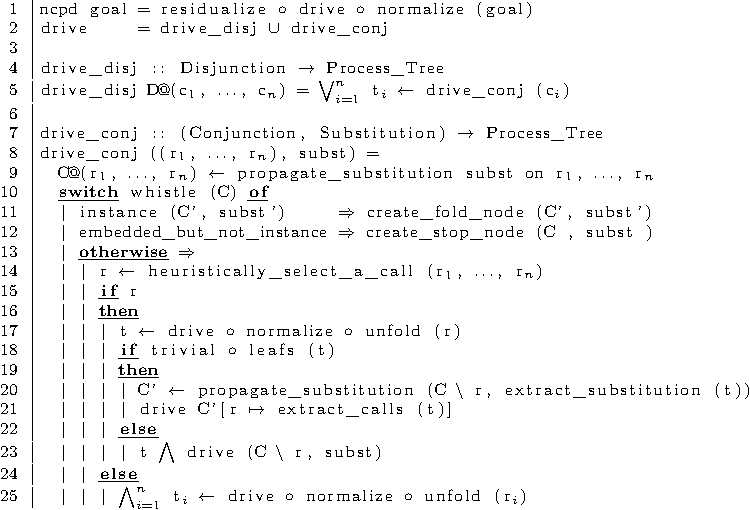
\includegraphics[width=0.7\textwidth]{algo_pseudo-crop.pdf}
  \caption{\db{Non-conjunctive Partial Deduction Pseudo Code}}
  \label{fig:ncpd-pseudo}
\end{figure}

In this section we will describe a novel approach to specialization of relational programs.
This approach draws inspiration from both conjunctive partial deduction and supercompilation.
The aim was to create a specialization algorithm which is simpler than conjunctive partial deduction and uses properties of \mk{} to improve performance of the input programs.
\db{The algorithm pseudocode is shown on Fig.~\ref{fig:ncpd-pseudo}\footnote{
    \db{For the sake of brevity and clarity, we provide functions \texttt{drive\_disj} and \texttt{drive\_conj} describing driving processes for disjunction and conjunction correspondingly.
      Driving itself is a trivial combination of presented functions (line 2)}}}.

The high-level idea behind the algorithm is to select a relation call to unfold by using a heuristic which decides if the call can narrow down the answer set \db{(line 15)}.
A driving tree is constructed for the selected call in isolation \db{(line 16)}.
The leaves of the computed tree are examined.
If all leaves are either computed substitutions or are calls to some relations accompanied with non-empty substitutions, then the leaves are collected and are put back into the root conjunction instead of the examined call \db{(lines 19,20)}.
According to denotational semantics of \mk{} it is safe to compute individual conjuncts in any order, thus it is ok to drive any call and then propagate its results onto the other calls.

A driving process creates a process tree, from which a residual program is later created.
The nodes of process tree include a \emph{configuraion} which describes the state of program evaluation at some point.
In our case configuration is a conjunction of relation calls.
The substitution computed at each step is also stored in the tree node, although it is not included into the configuration.

Each time we examine a conjunction of calls, we \emph{split} them into separate nodes which are driven independently from each other.
Among the relation calls we select one which is according to the heuristic is likely to narrow down the answer set \db{(line 15)}.
If the selected call does not suit the criteria, the results of its unfolding is not propagated onto other relation calls withing the conjunction and the next suitable call is selected \db{(line 22)}.

This process does create branchings whenever a disjunction is examined \db{(lines 4--6)}.
At each step we make sure that we do not start driving a conjunction which we have already examined.
To do this, we check if the current conjunction is renaming of any other configuration in the tree \db{(line 12)}.
If it is, then we create a special node which then is residualized into a call to the suitable relation.

We decided not to do generalization in this approach.
The generalization is used in supercompilation and partial deduction to ensure termination at the same time as some degree of specialization.
The generalization of two terms is usually a \emph{most-specific generalization}.
Generalization is used to abstract away some information computed during driving.
In conjunctive partial deduction generalization is modified to support treating of conjunctions.
The generalization selects subconjuctions of two conjuncts which are similar (call to the same relation and their arguments have similar shape and distribution).
For the subconjunctions selected a most-specific generalization is computed.

In our approach we only do splitting of a conjunction into individual relation calls.
This makes any program with an accumulating parameter to be a problem.
Sometimes when there is a need to do a proper generalization, it is in reality just an instance of some other goal within the tree and we can simply create a call there \db{(line 13)}.
Otherwise we are unable to meaningfully specialize such goal, but we can always just include the initial program in the residual program and call the corresponding relation.


\subsection{Unfolding}

Unfolding is a process of substitution of some relation call by its body with simultaneous computation of unifications.
To unfold a relation call we do the following steps.
First, the formal arguments of a relation are substituted for the actual arguments of the call in the body.
All fresh variables get instantiated.
The body is transformed into a canonical form (disjunction of conjunctions of either calls or unifications).
All unifications are computed.
Those disjuncts in which unifications fails are removed.
Other disjuncts take form of a conjunction of relation calls accompanied with a substitution.

The most important question is when to unfold.
Unfortunately, too much unfolding is sometimes is even worse than not enough unfolding.
There is a fine edge between those.
This problem is mentioned in the (CONTROL PAPER).
We believe that the following heuristic provides a reasonable control.

\subsection{Heuristic}

The intuition behind the heuristic is to find those calls which are safe to unfold.
We deem every static conjunct (non-recursive) to be safe because they never lead to growth in the number of conjunctions.
Those calls which unfold deterministically, meaning there is only one disjunct in the unfolded relation, are also considered to be safe.

The other more complicated case is when there are less disjuncts than there can possibly be.
This signifies that at least one branch of computations is gotten rid of.

The final heuristic selects the first conjunct which suites either of the following cases.
First we unfold those conjuncts which are static.
Then --- deterministic.
Then those which are less branching.
The last to be unfolded are those calls, which unfold to a substitution with not conjunction.

\subsection{Residualization}

Residualization is quite straightforward.
A branching in the process tree becomes a disjunction.
A split node becomes a conjunction.
Computed substitution is residualized as a conjunction of unifications.
A renaming node is just a call to a relation.
Relations are created for configurations on which leaf nodes are renamed.

One other thing is that when some configuration is occurred within the tree which is an instance of a configuration for which a new relation is created, then we just create a call.
